\title{Developing a Robust Algorithm to Measure\\Geometric Distortion in Imaging Systems}
\author{
J. David Giese\\Innolitics, LLC
\and
Yujan Shrestha, M.D.\\Innolitics, LLC
\and
Mircea Lazea\\CIRS, Inc.
}
\date{\today}

\documentclass[12pt]{article}

\usepackage{amsmath, amssymb, amsbsy, cite, graphicx, subcaption}
\usepackage[font={footnotesize}]{caption}

\begin{document}
\maketitle

\section{Introduction}
MR scanners can introduce geometric distortion into their images.  For many clinical needs, these distortions are not relevant---for others they are relevant and worth measuring and correcting.  A detailed discussion of the causes of geometric distortion in MRIs and the applications in which they matter is beyond the scope of this report \cite{baldwin2007,torfeh2015,wang2005,mribook}.  

Geometric distortion in MR scanners is typically measured using images of specially constructed grid phantoms. By comparing the location of the phantom features in the image to their known locations in the phantom, one can calculate the geometric distortion introduced by the scanner into the image.

This report presents our approach to developing a robust algorithm to measure geometric distortion from grid phantom images. The first section discusses the problem the algorithm is solving and introduces our terminology and assumptions.  The second section presents the framework we are using to validate and improve our algorithm.  The third section presents an overview of our current algorithm.  The final section presents preliminary results, discusses the limitations of our current algorithm, and suggests directions for future improvement.

\section{Problem}
Measuring the geometric distortion from a grid phantom image is a fiducial-based non-rigid registration problem \cite{hill2001}.  The goal is to register the distorted MRI of a grid phantom with an undistorted image of the same phantom.

The undistorted image can be a CT image or can be derived from knowledge of the phantom's construction. In either case, it must be assumed that no distortions are present.

The registration produces a transformation which maps locations in the distorted image to locations in the undistorted image.  The transformation will contain a rigid component (translation and rotation) and a non-rigid component.  The rigid component is assumed to originate from misalignment of the phantom within the scanner while the non-rigid component is a measurement of the geometric distortion.  In our algorithms, the rigid registration is performed, and then the rigidly registered fiducials are used to compute geometric distortion.  Figure \ref{fig:problem-overview} demonstrates the registration process with an example image.

\begin{figure}
    \centering
    \includegraphics[width=\linewidth]{problem-overview.pdf}
    \caption{The geometric distortion is the non-rigid component of the registration between the distorted and undistorted images of a grid phantom. \textbf{(a)} The undistorted image---this could be a CT or an image derived from a CAD model of the phantom.  \textbf{(b)} The distorted image of a phantom---usually an MRI of the phantom.  \textbf{(c)} The images (a) and (b) overlaid without any registration.  \textbf{(d)} A rigid registration is applied to (b) which is then overlaid onto (a).  The rigid registration negates any alignment errors introduced while positioning the phantom in the scanner. \textbf{(e)} A detail of (d) highlighting the displacement between fiducials in the undistorted image (squares) and the fiducials in the distorted image (circles).  The remaining distortion between the two images would be corrected by a full non-rigid registration. \textbf{(f)} The geometric distortion can be interpolated from the non-rigid component of the registration.}
    \label{fig:problem-overview}
\end{figure}

There are three stages to a generic algorithm that solves this registration problem.  The first stage locates fiducials in the distorted and undistorted images.  The second stage performs rigid registration between the sets of fiducials derived from both images while simultaneously matching corresponding fiducials.  The third stage calculates the geometric distortion (a simple subtraction) from the matched fiducials and interpolates them onto a grid.  Hence, the final output of the algorithm is a sampled vector field of geometric distortion within the scanner.  This vector field can be visualized and characterized in a variety of ways, e.g. according to the NEMA MS 12 standard \cite{nema2010}.  Figure \ref{fig:generic-algorithm} is a block diagram of the generic algorithm.

\begin{figure}
    \centering
    \includegraphics[width=\linewidth]{generic-algorithm.pdf}
    \caption{A generic representation of the problem we are solving.  Our algorithm must first detect the fiducials from the distorted image and the undistorted image (if we don't know their location up front). Then we apply a rigid registration to remove alignment errors (see Figure \ref{fig:problem-overview}d). The rigidly-registered distorted fiducials can be compared with the undistorted fiducials to interpolate the geometric distortion vector field.  Note that red squares represent images, orange squares point sets, and blue squares are vector fields.}
    \label{fig:generic-algorithm}
\end{figure}


\subsection{Assumptions}

Generic non-rigid registration is an open research area with many unsolved problems. To make our problem tractable, we make the following assumptions: 

\begin{enumerate}
\item The phantom has consistently oriented and formed features that can be identified using a convolution kernel.  As an example, a phantom that contains a Cartesian grid of intersecting cylindrical rods satisfies this assumption.

\item The fiducial locations in the undistorted image are known.  In Figure \ref{fig:problem-overview}e, this means we know the square locations without having to extract them from Figure \ref{fig:problem-overview}a.  In Figure \ref{fig:generic-algorithm}, this means we do not need to detect features in the undistorted image. This assumption is satisfied because we either know the fiducial locations from knowledge of the phantom's construction, or we can detect the phantom feature locations from a CT image of the phantom assumed to have no distortion.

\item The images are sufficiently resolved such that the phantom fiducials are detectable.  In the case of a phantom with cylindrical grid intersections, this means that the pixel spacing along all three dimensions is smaller than the intersecting rods.

\item The scanner introduces minimal geometric distortion near its isocenter.  This assumption is reasonable for certain MR scan parameters.  For example, automatic shimming will increase the homogeneity of the static magnet near the isocenter, but this setting can be turned off \cite{baldwin2007}.

\item The images are crudely registered.  In particular, we assume the magnitude of the translation component of the registration is less than the grid phantom spacing.  We also assume the rotation component is less than a few degrees.
\end{enumerate}

\subsection{Terminology}

We denote the set of fiducial locations in the undistorted image as $A$ and the set of fiducial locations in the distorted image as $B$.  The isocenter of the scanner defines the origin of $B$'s coordinate system.  The location of the origin in $A$ is generally different due to positioning errors, and the axes of $A$ and $B$'s coordinate systems are generally not oriented with one another.

The second stage of our generic algorithm applies a rigid registration so that $A$ and $B$ can be compared directly.  Rigidly registering $A$ and $B$ involves determining the six free variables---$x$, $y$, $z$, $\theta$, $\phi$, and $\xi$---which define the affine transformation matrix S.  We define this matrix as

\begin{equation*}
    \mathrm{S} = \mathrm{R}_x(\theta) \cdot \mathrm{R}_y(\phi) \cdot \mathrm{R}_z(\xi) \cdot \mathrm{T}(x, y, z)
\end{equation*}

where

\begin{align*}
    \mathrm{R}_x(\theta) =&
    \begin{bmatrix}
        1 & 0 & 0 & 0\\
        0 & \cos(\theta) & -\sin(\theta) & 0\\
        0 & \sin(\theta) & \cos(\theta) & 0\\
        0 & 0 & 0 & 1\\
    \end{bmatrix},&
    \mathrm{R}_y(\phi) =&
    \begin{bmatrix}
        \cos(\phi) & 0 & \sin(\phi) & 0\\
        0 & 1 & 0 & 0\\
        -\sin(\phi) & 0 & \cos(\phi) & 0\\
        0 & 0 & 0 & 1\\
    \end{bmatrix},
    \\
    \mathrm{R}_z(\xi) =&
    \begin{bmatrix}
        \cos(\phi) & \sin(\phi) & 0 & 0\\
        -\sin(\phi) & \cos(\phi) & 0 & 0\\
        0 & 0 & 1 & 0\\
        0 & 0 & 0 & 1\\
    \end{bmatrix},&
    \mathrm{T}(x, y, z) =&
    \begin{bmatrix}
        1 & 0 & 0 & x\\
        0 & 1 & 0 & y\\
        0 & 0 & 1 & z\\
        0 & 0 & 0 & 1\\
    \end{bmatrix}.
\end{align*}

We refer to the set of points in $A$ that have been rigidly registered to $B$ as $A_\textrm{S}$.  We have

\begin{equation*}
    A_\textrm{S} = \left\{ \mathbf{a}_\textrm{S} \;\; \Big| \;\; \begin{bmatrix} \mathbf{a}_\textrm{S} \\ 1 \end{bmatrix} = \mathrm{S} \cdot \begin{bmatrix} \mathbf{a} \\ 1 \end{bmatrix} , \;\; \mathbf{a} \in A \right\}.
\end{equation*}

It is useful to categorize the points in $A$ and $B$.

\begin{enumerate}
    \item Points in $B$ that correspond to points in $A$ are referred to as \textit{matching points} or \textit{true positives}.
    \item Points in $B$ that do not correspond to points in $A$ are \textit{false positives}.
    \item Points in $A$ that do not have a corresponding point in $B$ are \textit{false negatives}.
\end{enumerate}

The problem of deciding how to match points is a particular instance of the ``correspondence problem'' that exists in many non-rigid registration problems \cite{hill2001}.  We consider two points, $\textbf{a} \in A$ and $\textbf{b} \in B$, to be matching if

\begin{enumerate}
    \item they are within a certain distance, $\rho(|\textbf{b}|)$, from one another
    \item neither point has already been matched
    \item matching them minimizes the total sum of distances of all matched points.
\end{enumerate}

The threshold distance, $\rho(|\textbf{B}|)$ is a monotonically increasing function of the distance of a point to the isocenter of the scanner.  It is loosely derived from our physical knowledge of the scanner.  For example, if $\rho(|\textbf{b}|) = 1 + 0.05 \times |\textbf{b}|$, then two points at the isocenter must be within 1mm to be considered matching. At 30cm from the isocenter, they must be within 16mm.

The form of $\rho$ is important.  A low threshold may prevent exceptionally distorted points from matching, resulting in false negatives.  A high threshold may allow false positives to match.  

Typically, each point in $A$ will be matched to the closest point in $B$. However, if there is a point in $B$ that could match multiples points in $A$, it will be matched with whichever point in $A$ minimizes the total sum of distances.  If there is a point in $B$ that is equidistant from two points in $A$ (both of which can only match this particular point), then the matching choice will be arbitrary.

We define $M$ to be the set of tuples of matched points, and $M_\textrm{S}$ as the set of tuples of matched and rigidly registered points

\begin{align*}
    M =& \; \{ (\mathbf{a}, \mathbf{b}) \; | \; \mathbf{a} \in A, \; \mathbf{a} \; \textrm{matches} \; \mathbf{b} \} \\
    M_\textrm{S} =& \; \{ (\mathbf{a}_\textrm{S}, \mathbf{b}) \; | \mathbf{a}_\textrm{S} \in A_\textrm{S}, \; \mathbf{a}_\textrm{S} \; \textrm{matches} \; \mathbf{b} \}.
\end{align*}

\section{Validation Framework}

It is deceptively easy to optimize an image processing algorithm to perform well on a particular image. Making it work well on a variety of images is more difficult because adjustments that improve its performance on one image often degrade its performance on another.  In order to escape a cycle of heuristic parameter tweaking on specific images, we built a validation framework that allows us to efficiently improve our algorithm's performance on many images.  As we collect more datasets from early customers and beta-testers, we hope to use this framework to further refine our algorithm until it works well with many phantoms and MRIs.

Our validation framework includes two ``tests'' and several visualization tools.  The first test validates the performance of all three stages of an algorithm.  The second test validates the performance of the feature detection stage in isolation.

The full algorithm test is more important because it quantifies the error in the geometric distortion, which is what end-users care about.  The feature detection  test is helpful for developers, but the metrics may be misleading.  For example, false positives returned from the feature detection algorithm may not affect the final distortion vector field if they can be identified and discarded.

\subsection{Full Algorithm Test}

The output of our algorithm is the geometric distortion vector field introduced by an MR scanner into an image.  Because we do not know the actual distortion field of a real MRI, we cannot directly verify our algorithm.  To work around this, we apply an artificial distortion to an existing MRI that we call the ``source image''.  In order to negate any existing geometric distortion, we annotate the fiducial locations in the source image.  Then we use these annotated points as the ``undistorted points'', $A$, in the algorithm.

Then we apply additional geometric distortion to the source image.  We may also add noise, amplitude fluctuations, rotations, or translations to the distorted image to validate our algorithm against challenging inputs.  Finally, we run our algorithm on the distorted image, using the annotated fiducials, and compare the resulting output against the original distortion field we applied.  The full algorithm test is illustrated in Figure \ref{fig:testing-setup}.

\begin{figure}
    \centering
    \includegraphics[width=\linewidth]{testing-setup.pdf}
    \caption{Our full algorithm test.  We apply a known distortion to an existing source image and feed the distorted image to our full algorithm.  We then compare the output to the known distortion field.  The smaller the mean target registration error, the better the more accurately our algorithm was able to measure the underlying distortion.}
    \label{fig:testing-setup}
\end{figure}

Annotating a source image is time consuming.  We tried existing tools, such as 3DSlicer, however they were too slow and inflexible.  Instead, we built a tool that allows us to quickly annotate images.  For example, we can annotate a large phantom MRI with thousands of points in about an hour.  This speed is possible because our annotation tool has custom keyboard shortcuts that make it very efficient to use.

The manually annotated fiducial locations have some error (errors are especially large along the slice-axis).  Grid-phantom features touching the outer edge of the phantom volume can be difficult to annotate because it is unclear whether the feature detection algorithm should be expected to identify them.

Once we have annotated a source image, we can generate many test cases from it by applying various combinations of distortions, rigid transformations, noise, and filters.  Figure \ref{fig:test-case} demonstrates a slice from an example test case with extreme distortion.

The final result of the test is the mean target registration error (TRE), which quantifies the disparity between the actual geometric distortion that we artificially introduced and the geometric distortion calculated by our algorithm \cite[page R37]{hill2001}.  If $\textbf{D}$ is the distortion calculated by our algorithm, and $\textbf{D}_a$ is the actual distortion, and $V$ is the volume over which we have a meaningful value, we have

\begin{equation*}
\textrm{TRE}_\textrm{mean} = \frac{1}{V}\int_V \| \textbf{D}(\textbf{r}) - \textbf{D}_a(\textbf{r}) \| d\textbf{r}.
\end{equation*}

A $\textrm{TRE}_\textrm{mean}$ of 0.2mm means that on average, our algorithm miscalculated the geometric distortion by 0.2mm.  Thus an end user interpreting the results returned from our algorithm may believe that the distortion is 0.2mm better or worse than it actually is.

$\textrm{TRE}_\textrm{mean}$ is a useful metric to quantify the performance of our algorithm, but it can be misinterpreted.  For example, our geometric distortion field may be wildly incorrect in a small portion of the volume.  If the remainder of the volume is reasonably accurate, the $\textrm{TRE}_\textrm{mean}$ may indicate that the algorithm is sufficiently precise on average that we do not notice the wildly inaccurate volume.  Additional metrics could help detect results such as this---for example, the maximum magnitude of the difference between the actual and calculated distortion fields.  But the best way to catch unusual cases is to visualize the three-dimensional fields.

\begin{figure}
    \centering
    \begin{subfigure}[b]{0.48\textwidth}
        \centering
        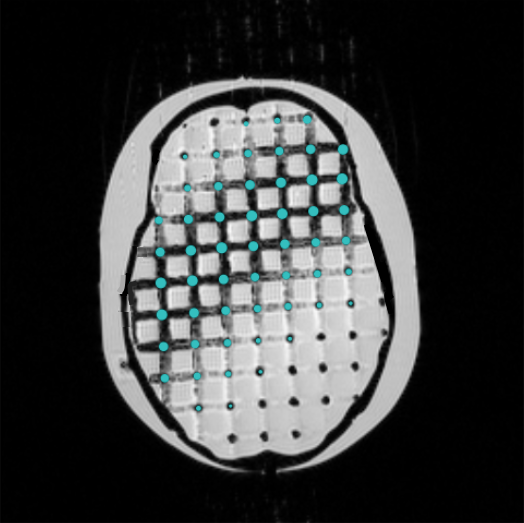
\includegraphics[width=\textwidth]{source-image.png}
        \caption{Source Image}
        \label{fig:test-case_1}
    \end{subfigure}%
    ~
    \begin{subfigure}[b]{0.48\textwidth}
        \centering
        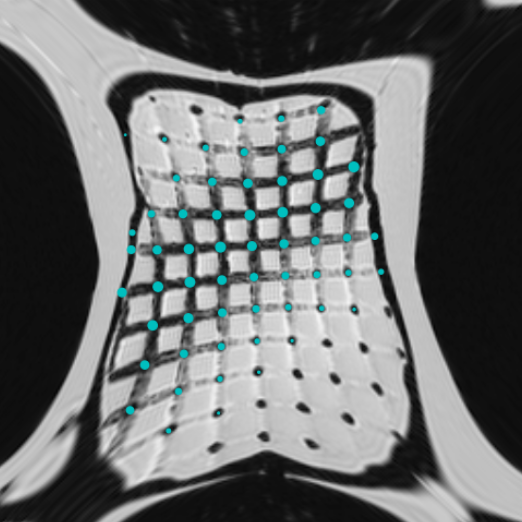
\includegraphics[width=\textwidth]{distorted-image.png}
        \caption{Distorted Image}
        \label{fig:test-case_2}
    \end{subfigure}
    \caption{Example test case with extreme distortion.  In order to validate our algorithm, we apply a known distortion to existing MRI source images. \textbf{(a)} Fiducials are manually annotated on the source image, and are overlaid as light blue circles.  The size of the circles indicates their position along the slice-axis (in or out of the page).  \textbf{(b)} The detected fiducials overload on the distorted image.}
    \label{fig:test-case}
\end{figure}

\subsection{Feature Detection Testing}

It is useful to have a separate test for feature detection because it is the most sensitive stage of the algorithm.  Furthermore, failures in the full algorithm test due to the feature detection stage likely won't provide enough insight to correct the problem.

The feature detection test begins by applying an artificial distortion to an existing image that has been annotated.  The distorted image is fed into the feature detection algorithm, which returns $B$.  Next, we apply the distortion to the set of annotated points, which we call $A$.  The meaning of $A$ in the context of this test is unusual.  It is useful to retain the same notation and matching algorithm, however, so we use $A$ instead of introducing new notation.

Typically there is an expected discrepancy between $B$ and $A$ (this is what we are measuring).  In the context of the feature detection test, if the feature detection is perfect then $B = A$.  Thus, it does not make sense to use our typical `rho`, and instead we use $\rho(|\mathbf{b}|) = 2$---hence points are categorized as false positives if they are further than 2mm apart.  

We quantify the performance of the algorithm using the following metrics: 

\begin{align*}
    \textrm{TPF} &= \frac{N_\textrm{TP}}{N_A} \\
    \textrm{FNF} &= \frac{N_\textrm{FN}}{N_A} \\
    \textrm{FPF} &= \frac{N_\textrm{FP}}{N_B} \\
    \textrm{FLE}_\textrm{mean} &= \frac{1}{N_\textrm{TP}} \sum_{(\textbf{a}, \textbf{b}) \in M} \| \textbf{a} - \textbf{b} \|\\
\end{align*}

The TPF, or True Positive Fraction, is the fraction of known fiducials that were successfully identified.  The FPF is the fraction of detected fiducials that were false positives.  The FNF is the fraction of known fiducials that were not identified.  Note that FNF + TPF = 1.  The $\textrm{FLE}_\textrm{mean}$ is the mean displacement between matched points, also known as the ``fiducial localization error'' \cite{hill2001}.

As is the case with the $\textrm{TRE}_\textrm{mean}$ and the full algorithm test, these metrics can be misleading.  For example, the TPF may be close to 1 but the $\textrm{FLE}_\textrm{mean}$ may be too large, or the FPF may be high but all of the false positives are irrelevant because they lie on the periphery of the image and will be ignored in subsequent stages.  Accordingly, we believe visualizing the results is the only foolproof way to validate test results.  Figure \ref{fig:feature-detection-run} demonstrates the results of running our feature detection algorithm against a CT and MRI test dataset.

\begin{figure}
    \centering
    \includegraphics[width=\linewidth]{testing-feature-detection.pdf}
    \caption{Our feature detection test.  Ultimately, the target registration error is the most meaningful metric \cite[page R38]{hill2001}, however, it is useful to understand how well the feature detection stage of the algorithm performed in isolation.  Our feature detection test quantifies what fraction of the fiducials were calculated (the TPF), the number of incorrectly identified fiducials (the FPF), and the mean error of the matched points (the mean FLE).}
    \label{fig:testing-feature-detection}
\end{figure}

\begin{figure}
    \centering
    \begin{subfigure}[b]{0.48\textwidth}
        \centering
        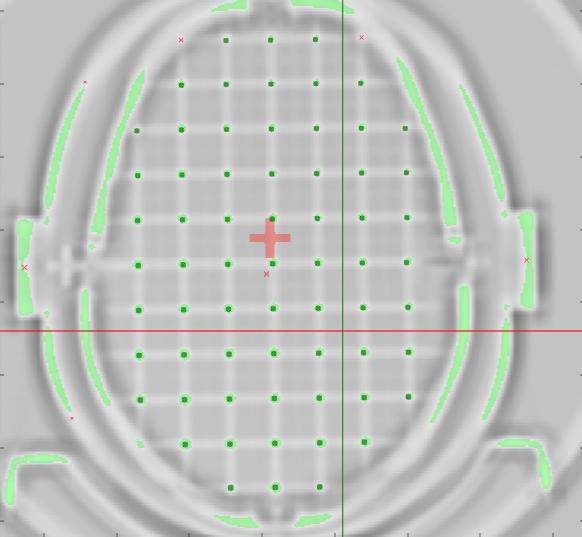
\includegraphics[width=\textwidth]{case-001-feature-detection.png}
        \caption{CT 604 Result}
        \label{fig:testing-feature-detection_1}
    \end{subfigure}%
    ~
    \begin{subfigure}[b]{0.48\textwidth}
        \centering
        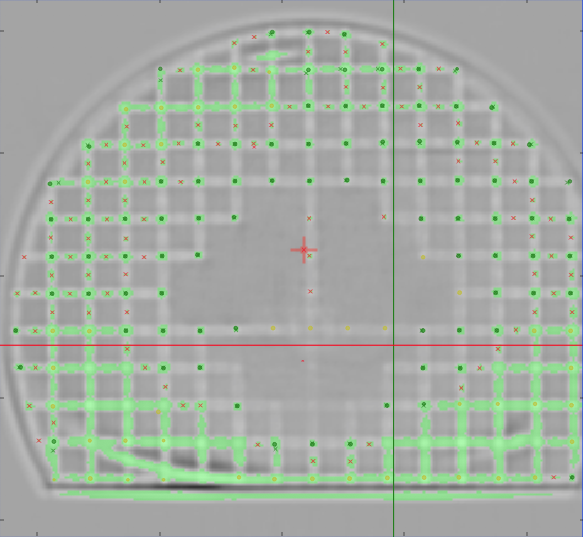
\includegraphics[width=\textwidth]{case-010-feature-detection.png}
        \caption{MRI 603A Result}
        \label{fig:testing-feature-detection_2}
    \end{subfigure}
    \caption{Results of running our feature detection test against an MR and CT source image.  The convolved image is placed in the background.  Green circles are true positives.  Red crosses are false positive.  Yellow circles are false negatives.  The light green overlay is the labeled binary mask used to detect features from the convolved image.  Our validation framework makes it very easy to quickly iterate on the algorithm and visualize how well it performed on various test cases.}
    \label{fig:feature-detection-run}
\end{figure}

\section{Current Algorithm}

Our algorithm combines our ideas with those found in the literature \cite{stanescu2010,baldwin2007}.  It is divided into the three general stages we outlined in Figure \ref{fig:generic-algorithm}: feature detection, rigid registration, and distortion interpolation.

\subsection{Feature Detection}

The goal of the feature detection stage is to localize the phantom grid intersections with sub-pixel precision.  Our algorithm consists of the following steps:

\begin{itemize}
    \item Invert the image if it is a CT (so that MRIs and CTs can be processed similarly).
    \item Convolve the image with a kernel shaped like the phantom's grid intersections.
    \item Localize peaks in the convolved image.
\end{itemize}

The grid intersection shape is known a priori.  For example, the CIRS 603A filter contains a grid of intersecting cylindrical beams.  The intersections are spaced 15mm from one another, and the beam's radius is 1.5mm.  Unfortunately, MRIs tend to distort the size of they phantom's grid cylinders.  A typical example of this phenomena is displayed in Figure \ref{fig:size-distortion}.  We compensate this effect in MRI images using multiplicative factor (e.g. of using 2mm instead of 1.5mm) when processing MR images; for CT images we use the physical cylinder radius.

\begin{figure}
    \centering
    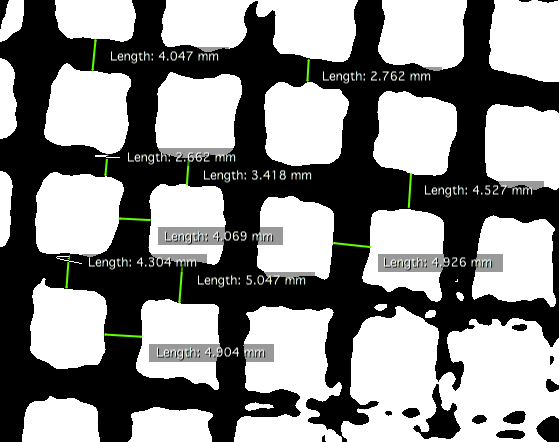
\includegraphics[width=\linewidth]{size-distortion.png}
    \caption{An MRI of a phantom with 3mm diameter grid cylinders.  The image was thresholded at a cutoff approximately halfway between the average value inside the cylinders and the average value outside the cylinders.  Multiple annotations highlight that the cylinder diameter in the images is usually larger than the actual phantom cylinder diameter.}
    \label{fig:size-distortion}
\end{figure}

It is important that the kernel be properly centered otherwise it will introduce a systematic shift into the detected feature locations.

Aliasing can degrade the algorithm's performance when the kernel's feature dimensions are on the scale of a pixel.  We perform a crude form of antialiasing by first constructing an upsampled version of the filter which we decimate using an averaging filter.  At high upsampling numbers, the kernel construction process uses a lot memory.  To alleviate the problem, we construct a single corner of the kernel, and then reflect it into the remaining seven corners.

The kernel is centered on a beam intersection, and its dimensions are approximately one grid-intersection spacing (e.g. 15mm).  A smaller kernel could also be used, however, the larger the kernel the better it will be able to differentiate grid intersections from other features in the image.

Figure \ref{fig:kernel} demonstrates the geometry of the grid intersection kernel.

\begin{figure}
    \centering
    \includegraphics[width=\linewidth]{kernel.pdf}
    \caption{Geometry of the grid intersection kernel construction.  A central slice of the 3D kernel is displayed.  The red area represents the cylindrical beams forming the grid.  Each side of the green quadrants is one half the intersection spacing.  The black rectangles indicate the locations of the kernel voxels.  The blue rectangles indicate the voxel locations in the upsampled image.  Note that the kernel size may be slightly larger than the intersection spacing.}
    \label{fig:kernel}
\end{figure}

The third stage, peak detection, involves several steps.

\begin{itemize}
    \item Build a spherical search neighborhood (a binary array) with a diameter of one grid-intersection spacing.
    \item Search throughout the convolved image for voxels whose value is equal to the maximum value within the search neighborhood.  The hight of this peak is the maximum value in the neighborhood less the minimum value within the neighborhood.
    \item Discard peaks that are near the edge of the image (these are usually due to border effects).
    \item Discard peaks corresponding to noise and other features in the phantom by discarding peaks whose height is less than 30\% the height of the 98th percentile height.
    \item Combine duplicate peaks that can occur if there are neighboring maximum values in the image.
    \item Perform some sort of sub-voxel peak detection using the initial set of peaks as seed locations.
\end{itemize}

Details of the last two steps need to be filled in once we have settled on an algorithm.

\subsection{Rigid Registration}

The goal of rigid registration is to find the ``best'' rigid registration matrix, $\textrm{S}$.  We mathematically define what it means to be the ``best'' by formulating a function, $f(S)$, whose minimum value selects the best metrics $S$.

The function $f$ should have the following properties:

\begin{enumerate}
\item It should minimize the distance between matching points in $A_\mathrm{S}$ and $B$.
\item It should maximize the number of matching points.  If we did not have this condition we could either not match any points or we could match a set of grid points that are shifted over by one or more $\Delta$s.
\item It should weight the distance between matching points near the isocenter more than points further away from the isocenter---the relative weighting can be characterized by a monotonically decreasing function $g(|\mathbf{b}|)$.
\item It should ignore any false positives.
\end{enumerate}

We can find $\mathrm{S}$ by minimizing the objective function:

\begin{equation*}
f(S) =
\sum_{(\textbf{a}_\textrm{S}, \textbf{b}) \in M_\textrm{S}} g(\left|\mathbf{b}\right|)
\;
(\left|\mathbf{b} - \mathbf{a}_\textrm{S}\right|/\rho(|\mathbf{b}|) - 1)
\;
u(\rho(|\mathbf{b}|) - \left|\mathbf{b} - \mathbf{a}_\textrm{S}\right|)
\end{equation*}

where $u$ is the Heaviside function.

Many distortion detection algorithms presented in the literature have not used the full set of points, $M$, and instead use a subset of the points located near the scanner's isocenter.  We believe that the main reason previous algorithms have limited the rigid registration to a subset of $M$, is because they are inappropriately minimizing over the distance squared \cite{wang2005}.  We believe it is beneficial to optimize over all of $M$ because it will help average out fiducial localization errors and any geometric distortion that may be present, even near the isocenter \cite{baldwin2007}.

We believe that it is inappropriate to use the distance-squared.  Doing so gives too much weight to distorted points and false-positive matches.  It also gives too little weight to points near the isocenter where distortion is low.  Many previous algorithms have circumvented these shortcomings by using a subset of $M$.  Instead of limiting $M$, we optimize over the distance and use a weighting function $g$ to decrease the weight of peripheral points.

We note that the L-$p$ norms with $p \in (0, 1]$ have been used in other registration applications with great success \cite{bouaziz2013}.  

\subsection{Distortion Interpolation}

The final stage of our algorithm is distortion interpolation.  This stage interpolates the rigidly-registered, matched points, $M_\textrm{S}$, onto a grid for simpler visualization and analysis.  We interpolate onto the voxel locations of the original MRI.  Points that can not be interpolated will be indicated using using floating point ``NaN'' values.  If the original MRI was an $n \times m \times k$ array, the distortion field will be a $n \times m \times k \times 3$ array.

We defined the distortion at $\mathbf{a}_\textrm{S}$ to be $\mathbf{D}(\mathbf{b}) = \mathbf{a}_\textrm{S} - \mathbf{b}$, where $(\mathbf{a}_\textrm{S}, \mathbf{b}) \in M_\textrm{S}$.  Note that there is an alternate definition that could be used.  In particular, $\mathbf{D}(\mathbf{a}_\textrm{S}) = \mathbf{a}_\textrm{S} - \mathbf{b}$.  The NEMA MS 12 standard's definition is ambiguous on which definition should be used \cite{nema2010}.  One can understand the difference between these definitions informally as follows.  The first definition represents how far the object in the distorted image was moved.  The second definition represents how far the underlying object at a location was moved.  The first definition is image-centric, the second object-centric.  We believe an image-centric definition is more useful because it allows one to overlay the distortion on the MRI and determine how far each pixel has been distorted.  Figure \ref{fig:interpolation} demonstrates the difference between the definitions.

\begin{figure}
    \centering
    \includegraphics[width=\linewidth]{interpolation.pdf}
    \caption{The distortion vector field can be interpolated from $M_\textrm{S}$ in two ways---by locating the error vector at $\mathbf{a}_\textrm{S}$ (orange) or at $\mathbf{b}$ (blue).  The choice of approach will determine the volume over which we can interpolate (indicated by the solid translucent overlays) as well as the interpolated values.}
    \label{fig:interpolation}
\end{figure}

The distortion is interpolated onto the grid by triangulating $M_\textrm{S}$ and performing linear barycentric interpolation on each triangle.

\section{Results and Discussion}

We have preliminary results, but not enough to present at this time.  We will be adding a results and discussion section soon.

\bibliographystyle{ieeetr}
\bibliography{./algorithm.bib}

\end{document}
